\documentclass[a4paper,14pt]{extarticle}
\usepackage[left=30mm, top=20mm, right=15mm, bottom=20mm, nohead]{geometry} 
\usepackage{cmap} % для кодировки шрифтов в pdf
\usepackage[T2A]{fontenc}
\usepackage[utf8]{inputenc}
\usepackage[english,russian]{babel}
\usepackage{graphicx} % для вставки картинок
\usepackage{amssymb,amsfonts,amsmath,amsthm,amsbsy} % математические дополнения от АМС
\usepackage{indentfirst} % отделять первую строку раздела абзацным отступом тоже
\usepackage{multicol}
\usepackage{tempora}
\usepackage{epstopdf}
\usepackage{mathtools}
\usepackage{framed}
\usepackage{wrapfig}
\usepackage{caption}
\usepackage{subcaption}
\usepackage{titlesec}
\usepackage{setspace}
\usepackage{float}
\usepackage{epstopdf}
\usepackage{hepunits}
\captionsetup[figure]{font=small,labelfont=small,name={Рис.},labelsep=period}
\titleformat{\section}
{\normalsize\bfseries} % format
{}                % label
{0pt}             % sep
{\Large}           % before-code
\renewcommand{\thetable}{\Roman{table}}
\begin{document}
	\selectlanguage{russian}
\newpage
% Ставим одинарный междустрочный интервал
\singlespacing
% Ставим геометрию для титульной страницы.
\newgeometry{left=3cm,right=1.5cm,top=2cm,bottom=2cm}

% Просто информация. Нигде в странице не используется, но зато попадёт в pdf info.
\author{Семенов А.\:В.}
\title{Измерение сечения e+ e- -> KS KL pi0}
\date{2017 г.}

\begin{titlepage}

%%%%%%%%%%%%%%%%%%%%%%%%%%%%%%%%%%%%%%%%%%%%%%%%%%%%%%%%%%%%%%%%%%%%%%%%%%%%%%%%

\begin{center}
    {\fnt{10.5} МИНИСТЕРСТВО ОБРАЗОВАНИЯ И НАУКИ РОССИЙСКОЙ ФЕДЕРАЦИИ} \\
        \vspace{0.3\baselineskip}
    {\fnt{10.5} ФЕДЕРАЛЬНОЕ ГОСУДАРСТВЕННОЕ АВТОНОМНОЕ ОБРАЗОВАТЕЛЬНОЕ \\ 
		\vspace{-0.3\baselineskip}
		УЧРЕЖДЕНИЕ ВЫСШЕГО ОБРАЗОВАНИЯ} \\
        \vspace{0.3\baselineskip}
    {\fnt{10.5} <<НОВОСИБИРСКИЙ НАЦИОНАЛЬНЫЙ ИССЛЕДОВАТЕЛЬСКИЙ ГОСУДАРСТВЕННЫЙ \\
		\vspace{-0.3\baselineskip}
		УНИВЕРСИТЕТ>> (НОВОСИБИРСКИЙ ГОСУДАРСТВЕННЫЙ УНИВЕРСИТЕТ, НГУ)}
\end{center}

%%%%%%%%%%%%%%%%%%%%%%%%%%%%%%%%%%%%%%%%%%%%%%%%%%%%%%%%%%%%%%%%%%%%%%%%%%%%%%%%

\vspace{0.5\baselineskip}

\noindent
{\fnt{11}Факультет}
$\overset{\text{\fnt{11}\textbf{ФИЗИЧЕСКИЙ}}\phantom{\hspace{10.9cm}}}{\underline{\hspace{0.88\textwidth}}}$

\vspace{0.3\baselineskip}

\noindent
{\fnt{11}Кафедра}
$\overset{\text{\fnt{11}\textbf{ФИЗИКИ ЭЛЕМЕНТАРНЫХ ЧАСТИЦ}}\phantom{\hspace{4.8cm}}}{\underline{\hspace{0.895\textwidth}}}$

\vspace{1\baselineskip}

\noindent
{\fnt{11}Направление подготовки}
$\overset{\text{\fnt{11}\textbf{03.03.02 ФИЗИКА}}\phantom{\hspace{8cm}}}{\underline{\hspace{0.73\textwidth}}}$

\vspace{0.3\baselineskip}

\noindent
{\fnt{11}Образовательная программа}
$\overset{\text{\fnt{11}\textbf{БАКАЛАВРИАТ}}\phantom{\hspace{7.3cm}}}{\underline{\hspace{0.69\textwidth}}}$

%%%%%%%%%%%%%%%%%%%%%%%%%%%%%%%%%%%%%%%%%%%%%%%%%%%%%%%%%%%%%%%%%%%%%%%%%%%%%%%%

\vspace{\baselineskip}

\begin{center}\bfseries
    {\fnt{11} ВЫПУСКНАЯ КВАЛИФИКАЦИОННАЯ РАБОТА БАКАЛАВРА} \\
\end{center}

%%%%%%%%%%%%%%%%%%%%%%%%%%%%%%%%%%%%%%%%%%%%%%%%%%%%%%%%%%%%%%%%%%%%%%%%%%%%%%%%

\vspace{0.3\baselineskip}

\noindent
$\overset{\text{\fnt{11}Семенов Александр Владимирович}}
{\underset{\text{\fnt{9}(фамилия, имя, отчество автора)}}{\underline{\hspace{\textwidth}}}}$

%%%%%%%%%%%%%%%%%%%%%%%%%%%%%%%%%%%%%%%%%%%%%%%%%%%%%%%%%%%%%%%%%%%%%%%%%%%%%%%%

\vspace{\baselineskip}

\noindent
{\fnt{11}Тема работы}
$\overset{\text{\fnt{11}Измерение сечения процесса e+e- -> KS KL pi0 с детектором КМД-3}}{\underline{\hspace{0.855\textwidth}}}$

\noindent
$\overset{}{\underline{\hspace{\textwidth}}}$

\noindent
$\overset{}{\underline{\hspace{\textwidth}}}$

%%%%%%%%%%%%%%%%%%%%%%%%%%%%%%%%%%%%%%%%%%%%%%%%%%%%%%%%%%%%%%%%%%%%%%%%%%%%%%%%

\vspace{2\baselineskip}

\noindent
\begin{tabular}{@{}p{0.5\textwidth}@{}@{}R{0.5\textwidth}@{}}
\fnt{11}\textbf{<<К защите допущена>>} &  \\
\fnt{11}Заведующий кафедрой,           & \fnt{11}\textbf{Научный руководитель} \\
\fnt{11}канд. физ.-мат. наук, доцент   & \fnt{11}канд. физ.-мат. наук, \\
\fnt{11}зав. лаб ИЯФ СО РАН            & \fnt{11}н.с. ИЯФ СО РАН\\
$\overset{\text{\fnt{11}Эйдельман, С.\,И.}}{\underset{\text{\fnt{8}(фамилия, И.\,О.)}}{\underline{\hspace{0.225\textwidth}}}}
\overset{\text{\fnt{11}/}}{}
\overset{\text{\fnt{11}}}{\underset{\text{\fnt{8}(подпись)}}{\underline{\hspace{0.125\textwidth}}}}$ &
$\overset{\text{\fnt{11}Шебалин, В.\,Е.}}{\underset{\text{\fnt{8}(фамилия, И.\,О.)}}{\underline{\hspace{0.225\textwidth}}}}
\overset{\text{\fnt{11}/}}{}
\overset{\text{\fnt{11}}}{\underset{\text{\fnt{8}(подпись)}}{\underline{\hspace{0.125\textwidth}}}}$ \\
$\overset{\text{\fnt{11}<<}}{}
\overset{\text{\fnt{11}}}{\underline{\hspace{0.05\textwidth}}}
\overset{\text{\fnt{11}>>}}{}
\overset{\text{\fnt{11}}}{\underline{\hspace{0.215\textwidth}}}
\overset{\text{\fnt{11}2017 г.}}{}$ & 
$\overset{\text{\fnt{11}<<}}{}
\overset{\text{\fnt{11}}}{\underline{\hspace{0.05\textwidth}}}
\overset{\text{\fnt{11}>>}}{}
\overset{\text{\fnt{11}}}{\underline{\hspace{0.215\textwidth}}}
\overset{\text{\fnt{11}2017 г.}}{}$ \\
& \\
& \fnt{11}\textbf{Консультант} \\
& \fnt{11}канд. физ.-мат. наук, \\
& \fnt{11}с.н.с. ИЯФ СО РАН\\
&
$\overset{\text{\fnt{11}Кардапольцев, Л.\,В.}}{\underset{\text{\fnt{8}(фамилия, И.\,О.)}}{\underline{\hspace{0.225\textwidth}}}}
\overset{\text{\fnt{11}/}}{}
\overset{\text{\fnt{11}}}{\underset{\text{\fnt{8}(подпись)}}{\underline{\hspace{0.125\textwidth}}}}$ \\
&
$\overset{\text{\fnt{11}<<}}{}
\overset{\text{\fnt{11}}}{\underline{\hspace{0.05\textwidth}}}
\overset{\text{\fnt{11}>>}}{}
\overset{\text{\fnt{11}}}{\underline{\hspace{0.215\textwidth}}}
\overset{\text{\fnt{11}2017 г.}}{}$
\end{tabular}

%%%%%%%%%%%%%%%%%%%%%%%%%%%%%%%%%%%%%%%%%%%%%%%%%%%%%%%%%%%%%%%%%%%%%%%%%%%%%%%%

\vspace{1.5\baselineskip}

\begin{flushright}
\fnt{11}
$\overset{\text{\fnt{11}Дата защиты: <<}}{}
\overset{\text{\fnt{11}}}{\underline{\hspace{0.05\textwidth}}}
\overset{\text{\fnt{11}>>}}{}
\overset{\text{\fnt{11}}}{\underline{\hspace{0.215\textwidth}}}
\overset{\text{\fnt{11}2017 г.}}{}$
\end{flushright}

%%%%%%%%%%%%%%%%%%%%%%%%%%%%%%%%%%%%%%%%%%%%%%%%%%%%%%%%%%%%%%%%%%%%%%%%%%%%%%%%

\vfill

\begin{center}
    \fnt{11} Новосибирск, 2017
\end{center}

\end{titlepage}

% Возвращаем всё назад: полуторный интервал и геометрию.
\onehalfspacing
\restoregeometry
\newpage
\chapter*{Введение}
\label{sec:intro}
Развитие экспериментальных методов ядерной физики привело к появлению большого количества детектирующих систем. Отдельно стоит выделить координатные детекторы, по которым до сих пор ведутся активные исследования. Главными направлениями являются повышение эффективности регистрации и пространственного разрешения \cite{shechtman}.
\par Широкое распространение новых материалов и методов их обработки многократно улучшило параметры имеющихся детектирующих устройств, а так же позволило создавать детекторы новых конструкций. Так в 1997 г. группа ученых из Европейского центра ядерных исследований (CERN) под руководством Ф.~Саули успешно применила концепцию газового электронного умножения в микроструктурах для создания координатных детекторов, которые получили название <<GEM-детекторы>> или газовые электронные умножители \cite{sauli}. Их отличительными особенностями являются сравнительная простота конструкции, коэффициент усиления вплоть до $10^6$, а так же высокая радиационная стойкость. Данный тип детекторов широко используется в таких экспериментах, как PHOENIX (Франция), COMPASS (Швейцария), а так же в составе детекторов LHSb, TOTEM (ЦЕРН) и КЕДР (ИЯФ СО РАН).
\par В ИЯФ микроструктурные детекторы применяются не только в составе детекторов для экспериментов в ФЭЧ (КЕДР, СНД и КМД-3), но и в различных системах, связанных с ними. Одной из таких систем является установка <<лазерный поляриметр>>. В  основе её работы лежит предложенный в 1975 г. в ИЯФ метод резонансной поляризации \cite{bukin}. Применяется данная система для прецизионного измерения энергии на коллайдере ВЭПП-4М.
\par В рамках работ по усовершенствованию <<лазерного поляриметра>> планируется установить новый координатный детектор. Для выполнения данной задачи было решено использовать GEM-детекторы \cite{Bobr}. В ИЯФ существует возможность изготовления таких детекторов с использованием GEM-электродов, производимых в CERN. Таким образом, возникает необходимость в исследовании новых моделей GEM-детекторов.
\par \textbf{Целью данной работы} являлось создание и исследование характеристик GEM-детектора для установки <<лазерный поляриметр>>. Понимание физических процессов работы детектирующей системы, организацию модуля сбора данных, а также особенностей их анализа дает наиболее полную информацию о точности измерений.  
Для достижения поставленной цели были сформулированы основные задачи, которые определили ключевые направления деятельности:
\begin{itemize}
    
    \item Изучение физических основ работы газовых электронных умножителей и основных схем GEM-детекторов
    \item Определение основных параметров, влияющих на коэффициент усиления детектора 
    \item  Установка, настройка и управление механизацией детектора
    \item Создание и отладка системы сбора и обработки данных.
    \item Проведение экспериментов на выведенном пучке, в ходе которых исследованы физические характеристики детектора
    \item Обработка и анализ полученных данных 
	
\end{itemize}
\newpage
\chapter{Поляризационные эффекты и их применение для определения энергии пучка}
\label{sec:respnant_dep}
\section{Радиационная поляризация}
Эффект самопроизвольной поляризации заряженных частиц в ускорителях был описан Соколовым и Терновым еще в 1963г \cite{SokolovTernov63}. Качественно данный эффект можно описать следующим обоазом: в магнитном поле $\vec{H}$ потенциальная энергия частицы с магнитным моментом  $\vec{\mu}$ выражается как: 
\begin{equation}
U = - (\vec{\mu}, \vec{H}).
\end{equation} 
В случае поляризации пучка в ускорителе, $\boldsymbol{H}$ есть ведущее поле. Минимум потенциальной энергии дает значение угла между магнитным моментом и ведущим полем, равное нулю. Магнитный момент и спин электрона противоположно направлены, следовательно состояние электрона в пучке, в котором спин и магнитное поле антипараллельны, более устойчиво.
\par В работе  \cite{sokolov} определены доли от общего числа электронов, имеющие поляризацию против и по направлению поля: 
\begin{multicols}{2}
	\noindent
	\begin{equation}
	n_{\uparrow\downarrow} = \frac{15+8\sqrt{3}}{30} \approx 0.962 
	\end{equation}
	\begin{equation}
	n_{\uparrow\uparrow} = \frac{15-8\sqrt{3}}{30} \approx 0.038
	\end{equation}
\end{multicols}
Можно заметить, что практические все электроны в пучке имеют спин, направленный против ведущего поля. 
\section{Метод резонансной деполяризации}
Еще одним эффектом, возникающим при движении частиц со спином в электромагнитных полях, является прецессия спина $\vec{S}$ вокруг направления ведущего поля $\vec{H}$. Уравнение движения спина:
\begin{equation}
\cfrac{d\vec{S}}{dt} = [\vec{\Omega},\vec{S}],
\label{eq:precession_full}
\end{equation}
где $\vec{\Omega}$ имеет следующий вид:
\begin{equation}
\vec{\Omega} = -\biggl(\frac{q_0}{\gamma}+q'\biggr) \vec{H} + \frac{\gamma}{\gamma + 1}q' (\vec{\upsilon},\vec{H})\vec{\upsilon}- \biggl(\frac{q_0}{\gamma+1}  + q'\biggr)[\vec{\mathcal{E}},\vec{\upsilon}].
\end{equation}%
Здесь $q_0$ и $q'$ соответственно нормальная и аномальная части гиромагнитного отношения, $\gamma$ --- релятивистский гамма--фактор, $\vec{\upsilon}$ --- скорость частицы, $\vec{\mathcal{E}}$ --- вектор электрического поля.
В наиболее простом случае, когда $(\vec{\upsilon}, \vec{H})$ и $[\vec{\mathcal{E}},\vec{\upsilon}]$ равны нулю, имеем только один член, определяющий прецессию спина в ведущем магнитном поле. Таким образом, уравнение \ref{eq:precession_full} принимает вид:
\begin{equation}
\cfrac{d\vec{S}}{dt} = -\biggl(\frac{q_0}{\gamma}+q'\biggr) [\vec{H}, \vec{S}].
\label{eq:precession}
\end{equation}%
Если выразить ведущее поле через частоту обращения пучков как: 
\begin{equation}
\vec{H} = \frac {\gamma mc}{e}\omega_r\vec{n}_H.
\label{eq:larmor_freq}
\end{equation}
Подставим \ref{eq:larmor_freq} в \ref{eq:precession} и проведем серию математических преобразований чтобы получить выражение для частоты прецессии спина:
\begin{equation}
\omega_s=  \omega_{r}\bigg(\frac{q'}{q_0}\frac{E}{mc^2}+1\bigg).
\label{eq:spin_freq}
\end{equation}
Если измерить $\omega_s$ и $\omega_{r}$, то можно определить энергию электрона $E$ т.к. остальные константы в выражении \ref{eq:spin_freq} известны. $\omega_{r}$ можно найти разными способами: прямым измерением с помощью pickup--станций, по частоте ускоряющего поля в резонаторе и т.д. Однако, определение $\omega_s$ является весьма нетривиальной задачей. 
\par Один из методов, с помощью которого можно косвенно измерить  $\omega_s$ по регистрации резонансной деполяризации предварительно поляризованного пучка частиц, был разработан в ИЯФ СО РАН в 1974 г. и детально описывается в \cite{skrinskii}. Идея метода заключается в воздействии на пучок переменного электромагнитного поля определенной частоты. Если выполняется резонансное условие:
\begin{equation}
\omega_s=  k\omega_{r} \pm \omega_d,
\end{equation}
где $\omega_d$ -- частота электромагнитного поля, то исходная поляризация пучка нарушается. Это можно определить любым поляризационно чувствительным методом. Проводя сканирование по $\omega_d$ и фиксируя момент деполяризации, можно определить $\omega_s$.
\par Приведем оценку точности данного метода. Для этого определим какова точность определения параметров, входящих в выражение \ref{eq:spin_freq}:
\begin{itemize}
	\item $\displaystyle \frac{\delta (q'/q_0)}{q'/q_0} = 2.24 \cdot 10^{-10} $ \cite{PDG}
	\item $\displaystyle \frac{\delta (mc^2)}{mc^2}= 6.06\cdot10^{-9} $ \cite{PDG}
	\item $\displaystyle \frac{\delta (\omega_r)}{\omega_r} = 10^{-12} ~???$
\end{itemize}
Можно заметить, что точность определения массы электрона вносит наибольший вклад в точность измерения энергии. Физическое ограничение для $\delta E/E$ устанавливается на уровне $10^{-8}$. Измерения, использующие метод резонансной деполяризации, являются на данный момент самыми точными в мире.
\section{Регистрация эффекта деполяризации}
Существует несколько методов, с помощью которых можно зарегистрировать момент деполяризации. Все они предполагают рассеяние электронов пучка на ядрах --- Моттовское рассеяние, на электронах этого же пучка --- Тушековское рассеяние, а также Комптоновское рассеяние на поляризованных фотонах. Первый метод малоэффективен ввиду отсутствия в вакуумной камере достаточного количества атомов, на которых рассеивался бы пучок. Установки, использующие эффект Тушековского или внутрисгусткового рассеяния широко используются на малых энергиях ($E < 2~\GeV$). Из-за того, что измеряемый эффект обратно пропорционален четвертой степени энергии пучка, то в области $\Upsilon$---резонанса его применение является малоэффективным.
\par В данном случае Комптоновское рассеяние поляризованных фотонов на пучке электронов является единственным методом, применимым в данном диапазоне энергий. Сечение рассеяния зависит как от поляризации электрона, так и от поляризации фотона. Идея метода заключается в следующем: если пучок электронов поляризован, то существует связь между направлением рассеяния фотонов и их поляризацией. Изменяя направление поляризации (используя например левоциркулярные и правоциркулярные лазерные пучки), можно регистрировать рассеяние преимущественно в верхнюю или нижнюю полуплоскость т.к. поляризация электронов вертикальная, а значит в системе существует выделенное направление. В таком случае величина измеряемого эффекта определяется формулой:
\begin{equation}
	\Delta y = \frac{\hbar \omega_0}{2 m_e c^2} \mathcal{P} \Delta V L,
\end{equation}
где $\omega_0$ -- частота падающего фотона, $\mathcal{P}$ -- поляризация электронного пучка, $\Delta V$ -- разница стоксовских параметров для циркулярно поляризованного пучка фотонов, $L$ -- расстояние от точки взаимодействия до точки регистрации рассеянного фотона. При деполяризации электронного пучка $\mathcal{P} = 0$, следовательно вертикальная асимметрия рассеяния фотонов пропадает. Чтобы это зарегистрировать, необходим координатный детектор с достаточным разрешением. В нём эффект деполяризации будет выглядеть как слияние двух отдельных пятен, расположенных друг над другом, в одно пятно. 


\newpage
\section{Предел Рейтера и его зависимость от электрического поля в индукционном промежутке}
\label{sec:raether_exp}
Существенным параметром для детекторов, построенных с использованием ГЭУ, является коэффициент усиления. Существует два основных пути достижения его требуемых значений: 
\begin{itemize}
	\item обеспечение высокой электрической прочности электрода ГЭУ и приложение к нему более высоких напряжений
	\item использование несколько последовательно расположенных ГЭУ
\end{itemize}
Каждый из них имеет свои ограничения на применимость. ТУТ ОПИСАТЬ ПРО ПЕРВЫЙ МЕТОД.\par
Последовательное расположение нескольких ГЭУ с одной стороны вызывает усложнение конструкции детектора и увеличение количества материала на пути частицы. С другой стороны, напряжение на каждом электроде будет существенно ниже, чем в случае с одним ГЭУ. Нами было выдвинуто предположение
\newpage
\vspace{24pt}
\chapter{Исследование физических характеристик детектора <<Лазерного поляриметра>>}
\section{Определение уровня шумов детектора}
\label{sec:noise_study}
\begin{figure}[H]
	\begin{center}
		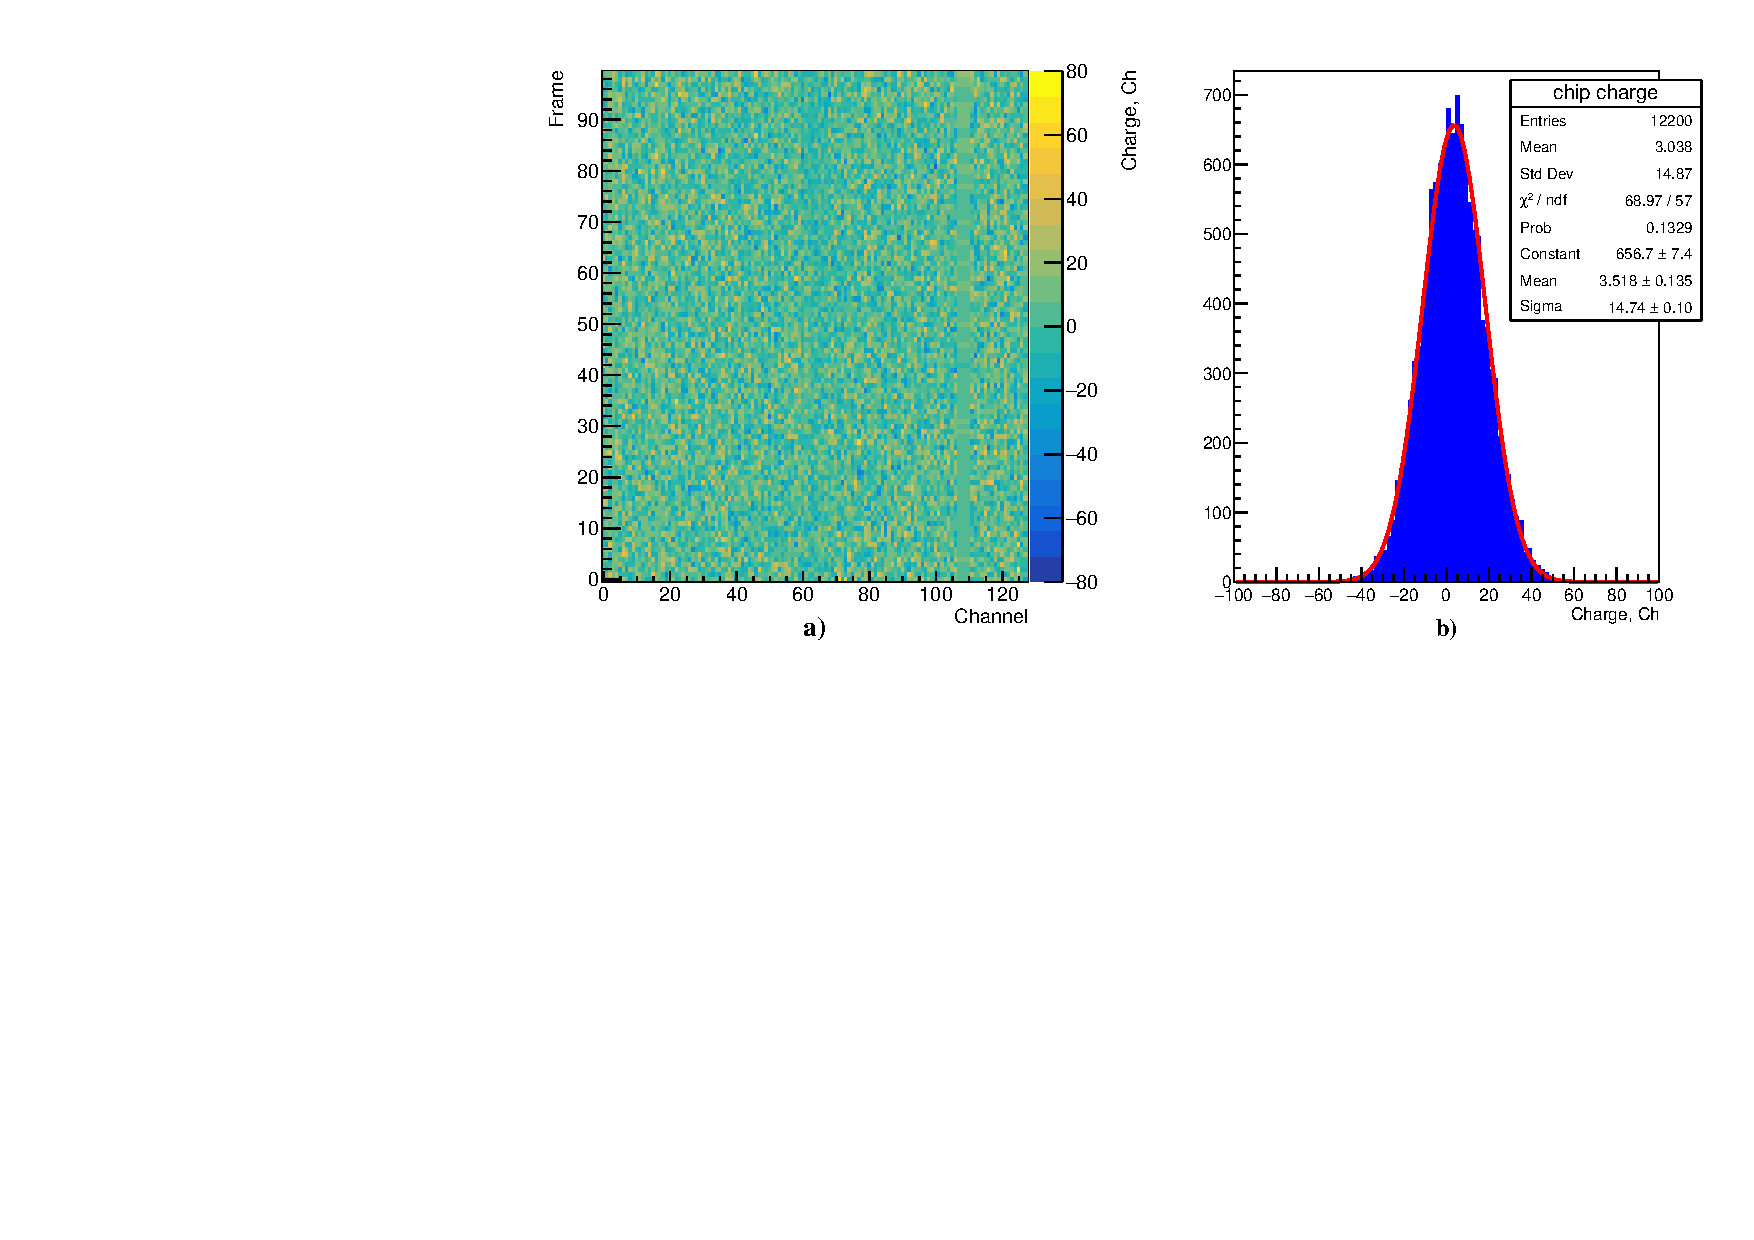
\includegraphics[width = 12cm, height = 6cm]{img/noise_map.pdf}
		\caption{a): Вид шумового события после вычитания пьедестала b): Распределение заряда в шумовом событии}
		\label{noise_map}
	\end{center}
\end{figure}
Рис. \ref{noise_map} показывает вид одного шумового события и распределение заряда в кадрах и каналах. Важным значением, которое можно извлечь уже из одного шумового события является уровень шумов. Его можно определить как корень из дисперсии распределения на Рис. \ref{noise_map} b). Шумы в данном эксперименте составили $\approx15$ каналов АЦП. Если взять несколько шумовых событий, то можно уточнить данное значение. Более того, записывая данные через равные промежутки времени, можно зафиксировать наличие дрейфа уровня шумов и их среднего значения. Такое исследование тоже было проведено. Для каждого набора данных существовала привязка по времени начала измерения. Чтобы определить, временной дрейф уровня среднего значения шумов, нами были Его результаты показали, что уровень шумов со временем меняется незначительно (Рис.\ref{fig:Noise_gr}.)

\begin{figure}[h]
	\centering
	\begin{subfigure}{.5\textwidth}
		\centering
		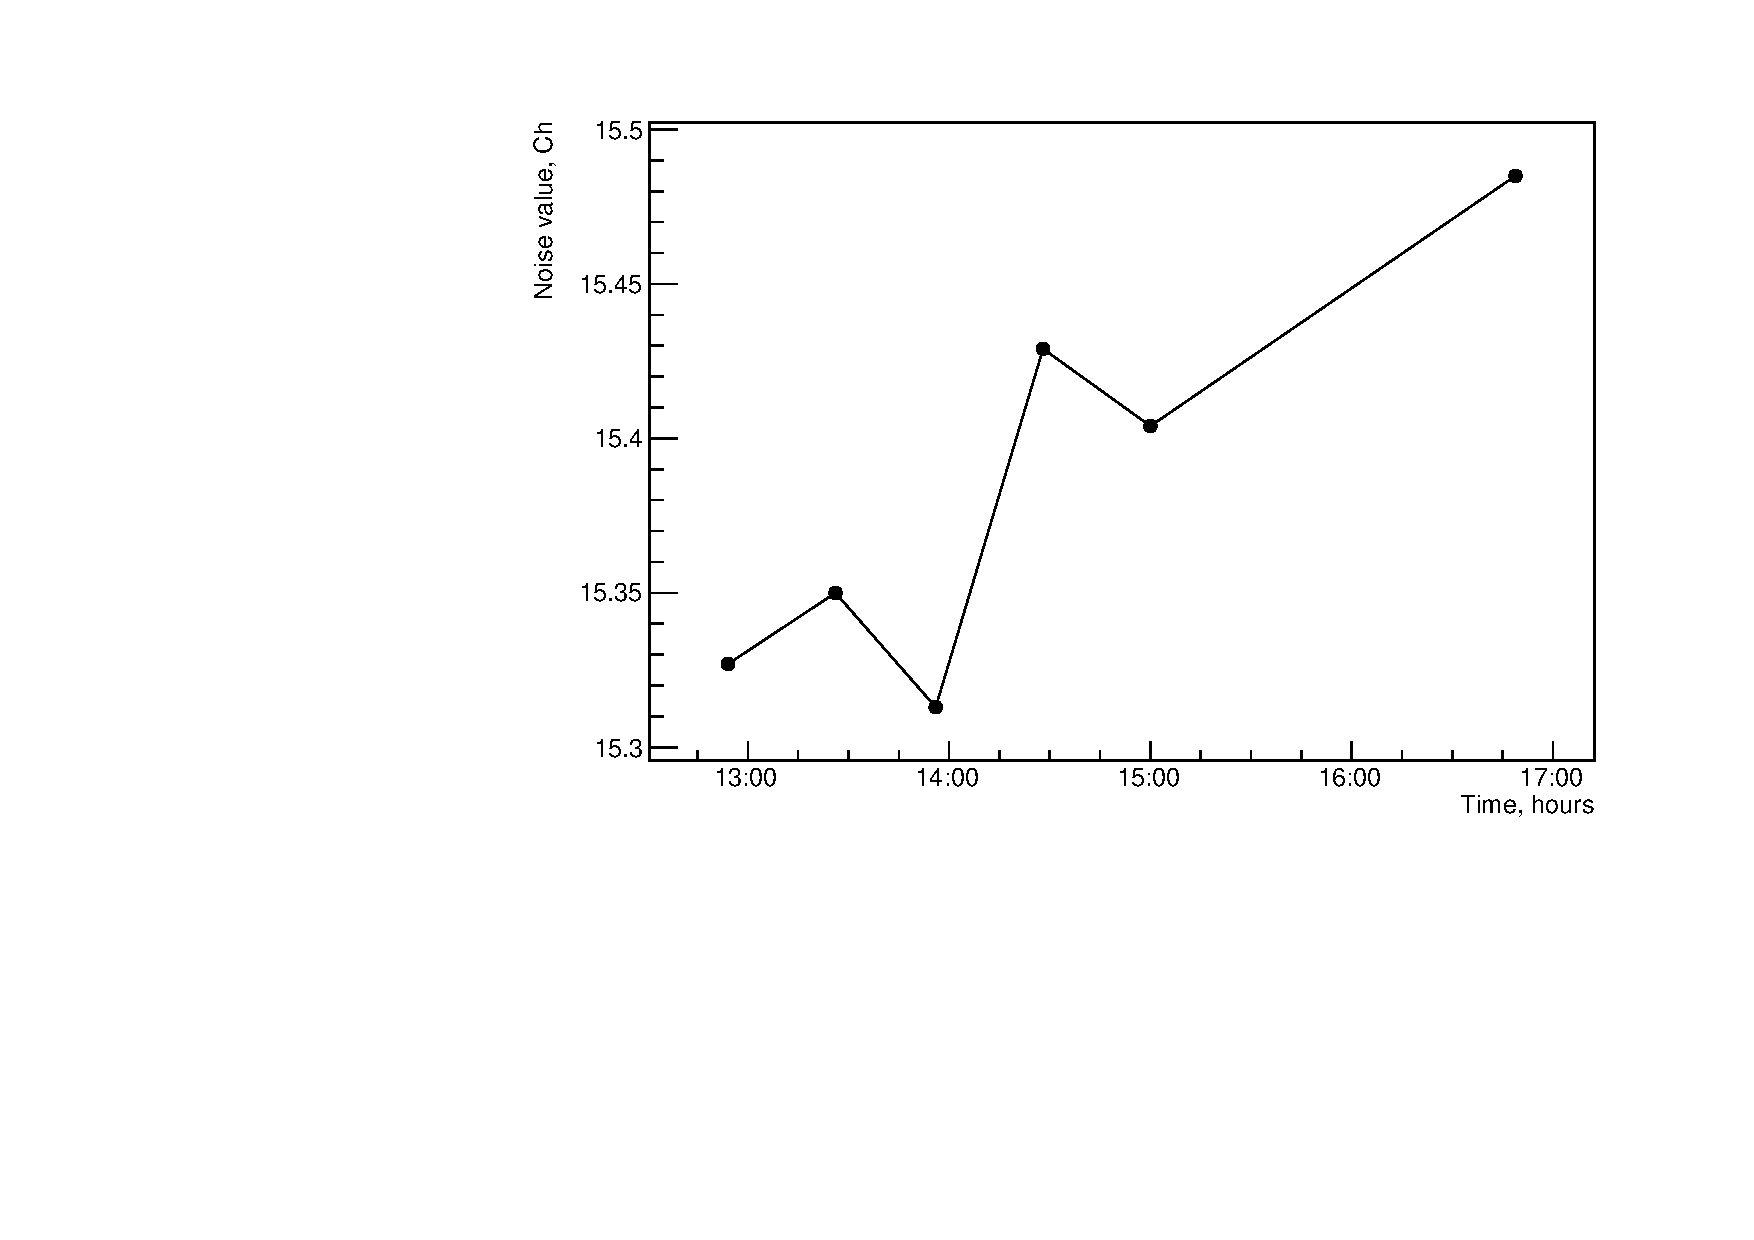
\includegraphics[width=1\linewidth]{img/Noise_time_drift.pdf}
		\caption{Уровень шумов}
	\end{subfigure}%
	\begin{subfigure}{.5\textwidth}
		\centering
		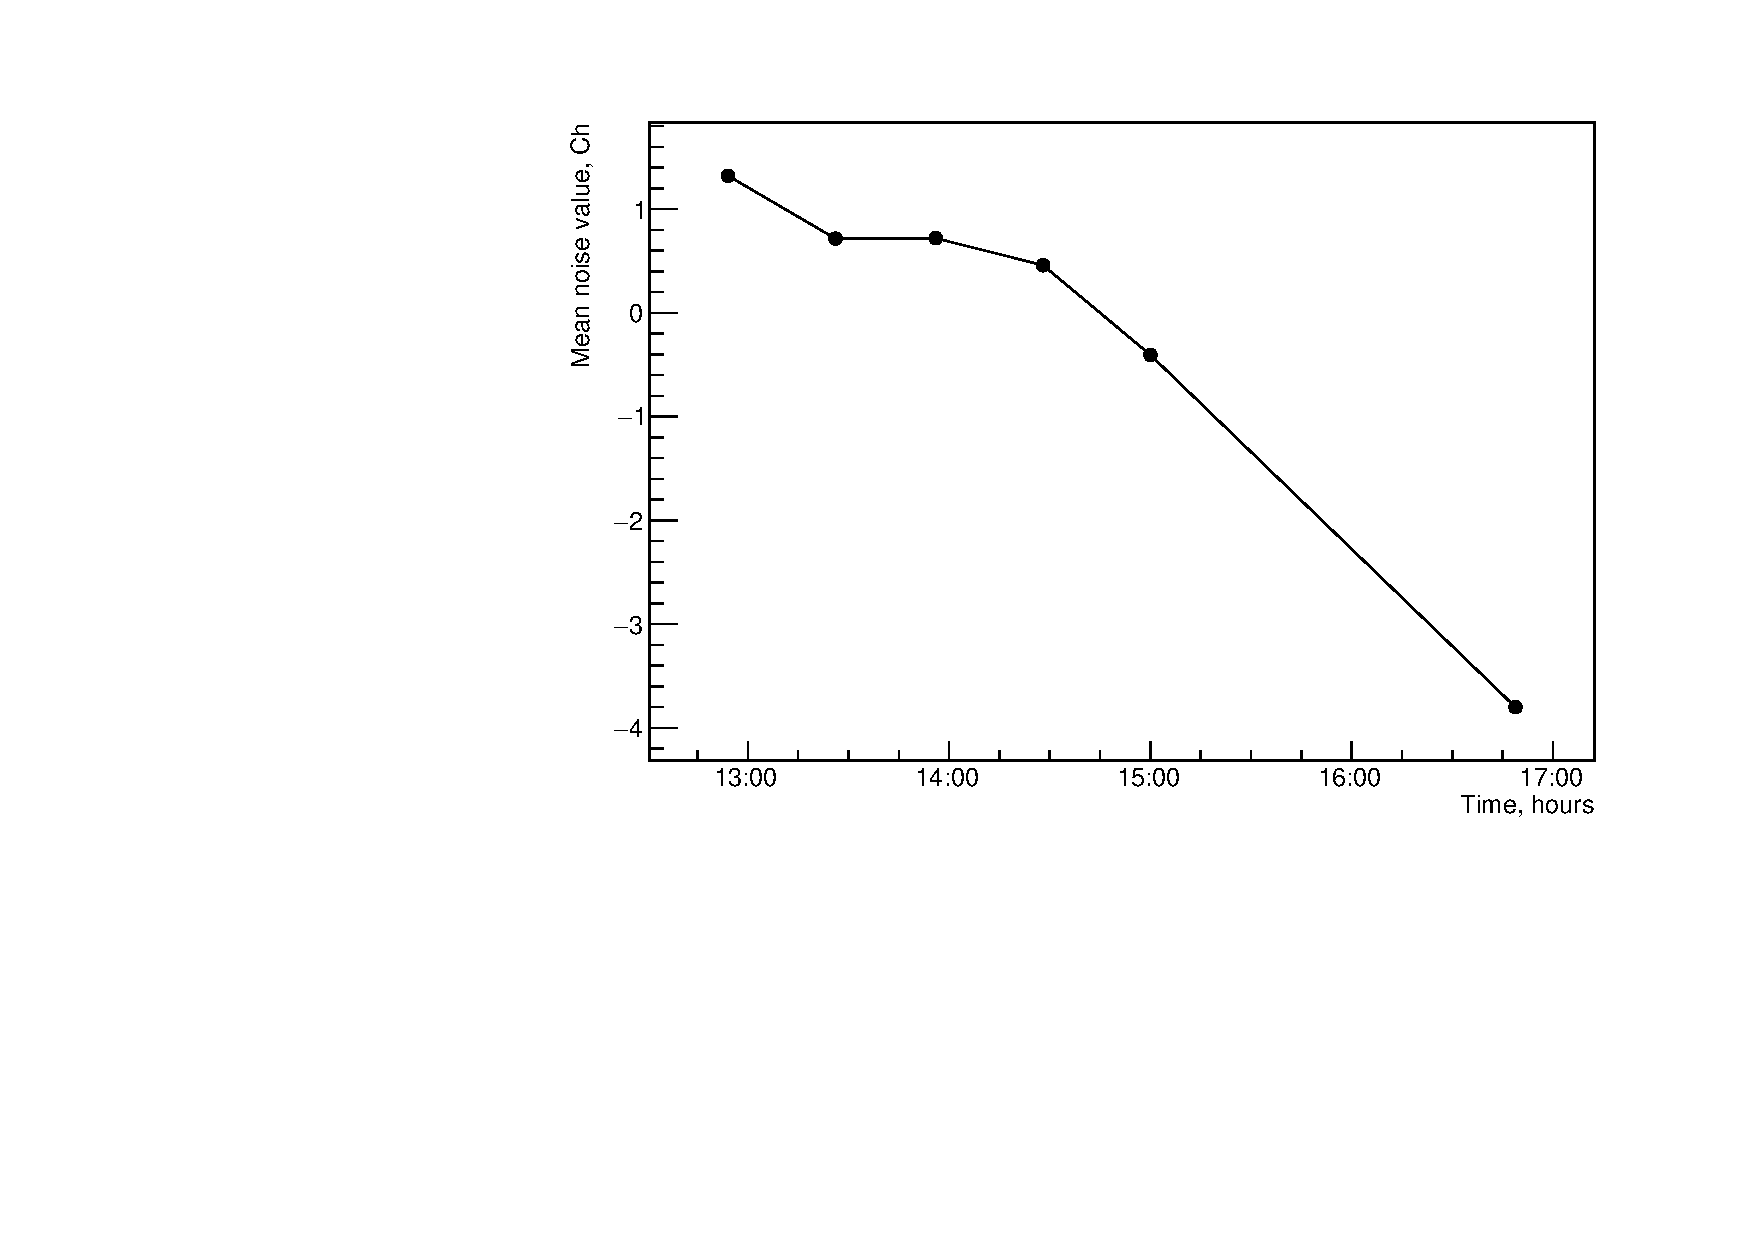
\includegraphics[width=1\linewidth]{img/Mean_time_drift.pdf}
		\caption{Среднее значение шума}
	\end{subfigure}
	\caption{Временной дрейф параметров шумовых событий: уровня шума и среднего значения шума. Каждая точка - среднее по $3\cdot10^7$ значений. В обоих случаях наблюдается линейный тренд. Статистические ошибки в точках малы и на графиках не видны}
	\label{fig:Noise_gr}
\end{figure}
Относительное изменение уровня шума за 4 часа составило $0.01~\sigma$, а дрейф среднего значения -- $0.33~\sigma$. Установившееся значение уровня шумов скорее всего зависит от температурного дрейфа электроники. Это является отдельной довольно обширной темой и в данной работе рассматриваться не будет. Однако, необходимы дополнительные долговременные эксперименты, которые смогут показать, каков максимально достижимый уровень шумов системы и насколько сдвигаются нулевые значения АЦП. Тем не менее, промежуточные результаты показали, что для <<Лазерного поляриметра>> это не является критичным.  
\section{Определение коэффициента усиления}
\label{sec:ampl_с}
При исследовании новой модели детектора необходимо различными методами проверить правильность работы, как ускоряющей структуры, так и вычитывающей электроники. Это можно сделать путём измерения коэффициента усиления детектора. 
%Стоит отметить, что зарегистрировать ионизацию первичной частицы достаточно сложно ввиду малого количества заряда. Для этого необходимы высокочувствительные АЦП. Однако, при использовании 
Коэффициент усиления в данной работе определяется как отношение зарегистрированного считывающей структурой заряда кластера к количеству частиц первичной ионизации, образованных в индукционном промежутке. 
Количество частиц первичной ионизации найдем, используя средние ионизационные потери и количество энергии, необходимое для образования ион--электронной пары. Известно, что потери энергии электронов в тонких слоях описываются модифицированной формулой Бете-Блоха:
\begin{equation}
\cfrac{dE}{dx} = \cfrac{2\pi N_0 e^4 Z\rho}{m_e c^2 \beta^2 A}\biggl[ln \bigg(\cfrac{ m_ec^2T\beta^2\gamma^2}{2I^2}\bigg) + f_{corr}(\beta)\biggr],
\label{eq:Bethe_Bloch}
\end{equation}
где $N_0$ -- число Авогадро, $e$ -- элементарный электрический заряд, $m_e$ -- масса электрона, $c$ -- скорость света, $\beta = v/c$ -- отношение скорости частицы к скорости света, $Z$ -- зарядовое число, $A$ -- массовое число, $\rho$ -- плотность вещества, $T$ -- кинетическая энергия электронов, $I$ -- энергия образования ион--электронной пары, $f_{coor}(\beta)$ -- функция, которая содержит поправки в случае $\beta \sim 1$. Параметры $A,Z,\rho$ относятся к веществу--радиатору т.е. к газовой смеси, которой заполнен детектор.
\par Вычисление показало, что средние потери энергии электронов с энергией $2.2~\MeV$ составляют $2.5~\keV/$см. Энергия образования одной ион--электронной пары в аргоне есть $26\eV$. Размер дрейфового промежутка -- 3 мм. Количество первичных электронов:
\begin{equation}
	N_e = \frac{dE/dx~\Delta x}{W} =\frac {2400~\eV/cm \cdot 0.3~cm}{26~\eV} = 28
\end{equation}
Зная средний заряд кластера $\langle Q\rangle$, можно определить коэффициент усиления системы GEM: 
\begin{equation}
K = \frac{\langle Q\rangle}{\langle N_e \rangle\ W},
\label{eq:ampl_k}
\end{equation}
где $I = 26~\eV$ -- средняя энергия образования ион-электронной пары в аргоне. 
\par Такой метод определения коэффициента усиления имеет один недостаток: в эксперименте определить средний заряд кластера достаточно трудно т.к. существуют ограничения электроники на максимальное измеренное значение. Более того, средний заряд кластера имеет распределение Ландау, параметром которого является наиболее вероятный заряд кластера. Поэтому вместо средних ионизационных потерь необходимо рассчитывать наиболее вероятные. Выражение для них можно записать следующим образом:
\begin{equation}
\Delta_p = \xi\biggl[ln \bigg(\cfrac{ m_ec^2T\beta^2\gamma^2}{2I^2}\bigg) + ln\bigg(\frac{\xi}{I}\bigg) + j - \beta^2 \biggr],
\label{eq:MP_energy_loss}
\end{equation}
где $j=0.2$, а параметр $\xi$ задается формулой:
\begin{equation}
\xi = 2\pi r_0^2 N_A m_ec^2\frac{Z}{A} \frac{\rho x} {\beta^2}, 
\end{equation}
где $r_0$ -- классический радиус электрона, $N_A$ -- число Авогадро. Оценка наиболее вероятных потерь в дрейфовом промежутке дает значение  $\Delta_p = 685~\eV$, а наиболее вероятное количество электронов $[N_e] = 26$, что на самом деле довольно близко к среднему значению.
%https://arxiv.org/pdf/1110.6761.pdf 
\subsection{Постановка эксперимента}
Для определения коэффициента усиления детектор облучался $2.2~\MeV$ электронами источника $Sr-90$, который располагался на герметичном кожухе детектора. Т.к. энергии электронов не хватало, чтобы пройти сквозь детектор, организация внешнего триггера по схеме совпадений не представлялась возможной. Поэтому запуск детектора проводился в автоматическом режиме.
\begin{figure}[H]
	\centering
	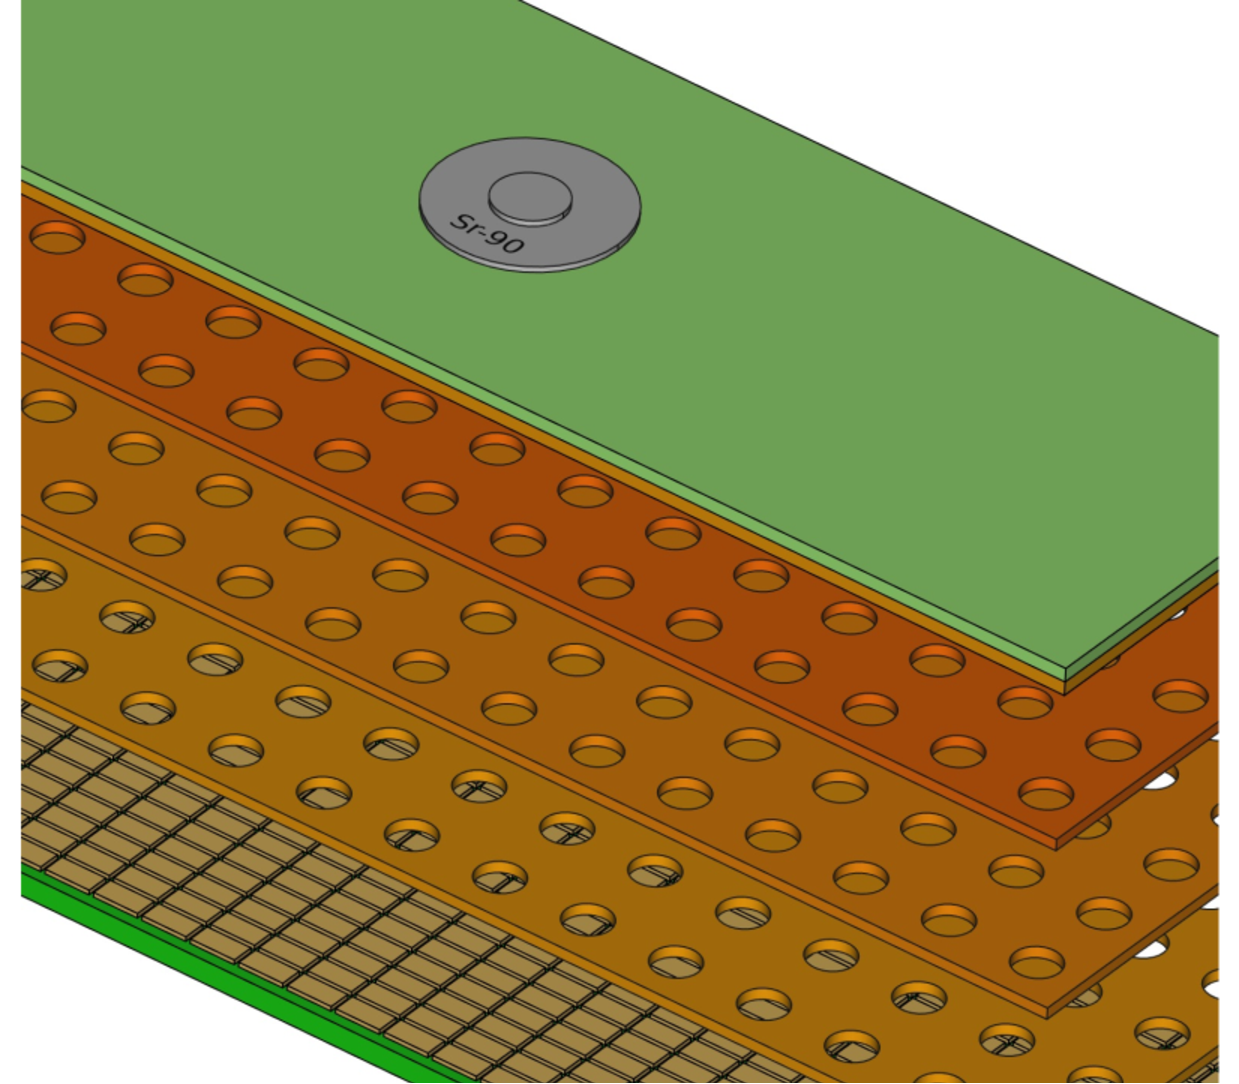
\includegraphics[height = 4 cm, width= 5.8cm]{img/GEM_Sr_source.pdf}
	\caption{Расположение источника относительно ускоряющей структуры}
	\label{fig:det_scheme+sr90}
\end{figure}
Электроны из источника проникали в газовый объем детектора и теряли энергию посредством ионизации. 
Первичная ионизация из дрейфового промежутка попадала в ускоряющую структуру, где происходило образование электронных лавин. Затем они проходили через два транспортных промежутка между GEM--электродами и попадали в индукционный промежуток. Заряд электронных лавин регистрировался считывающей структурой. По рассчитанному выше значению первичной ионизации и среднему заряду кластера определялся коэффициент усиления детектора. Цель эксперимента: проверить зависимость коэффициента усиления от напряжения. Для корректно работающей усиливающей и считывающей систем данная зависимость должна быть иметь экспоненциальный рост с увеличением напряжения. Набор статистики проходил в 7 точках по напряжению на ускоряющей структуре: от 3100 до 3450 В.

\subsection{Обработка и анализ полученных данных}
Полученные сырые данные обрабатывались с использованием алгоритмов, описанных в пункте \ref{sec:event_analysis}. После этого для каждого набора событий были построены распределения по заряду в кластерах. Для нахождения наиболее вероятного значения заряда экспериментальные гистограммы подгонялись функцией Ландау. После перевода каналов АЦП в единицы заряда коэффициент усиления находился по формуле \ref{eq:ampl_k}. На Рис. \ref{fig:charge_landau} можно видеть распределения по заряду кластера для двух точек по напряжению. 
\begin{figure}[h]
\centering
\begin{subfigure}{.45\textwidth}
	\centering
	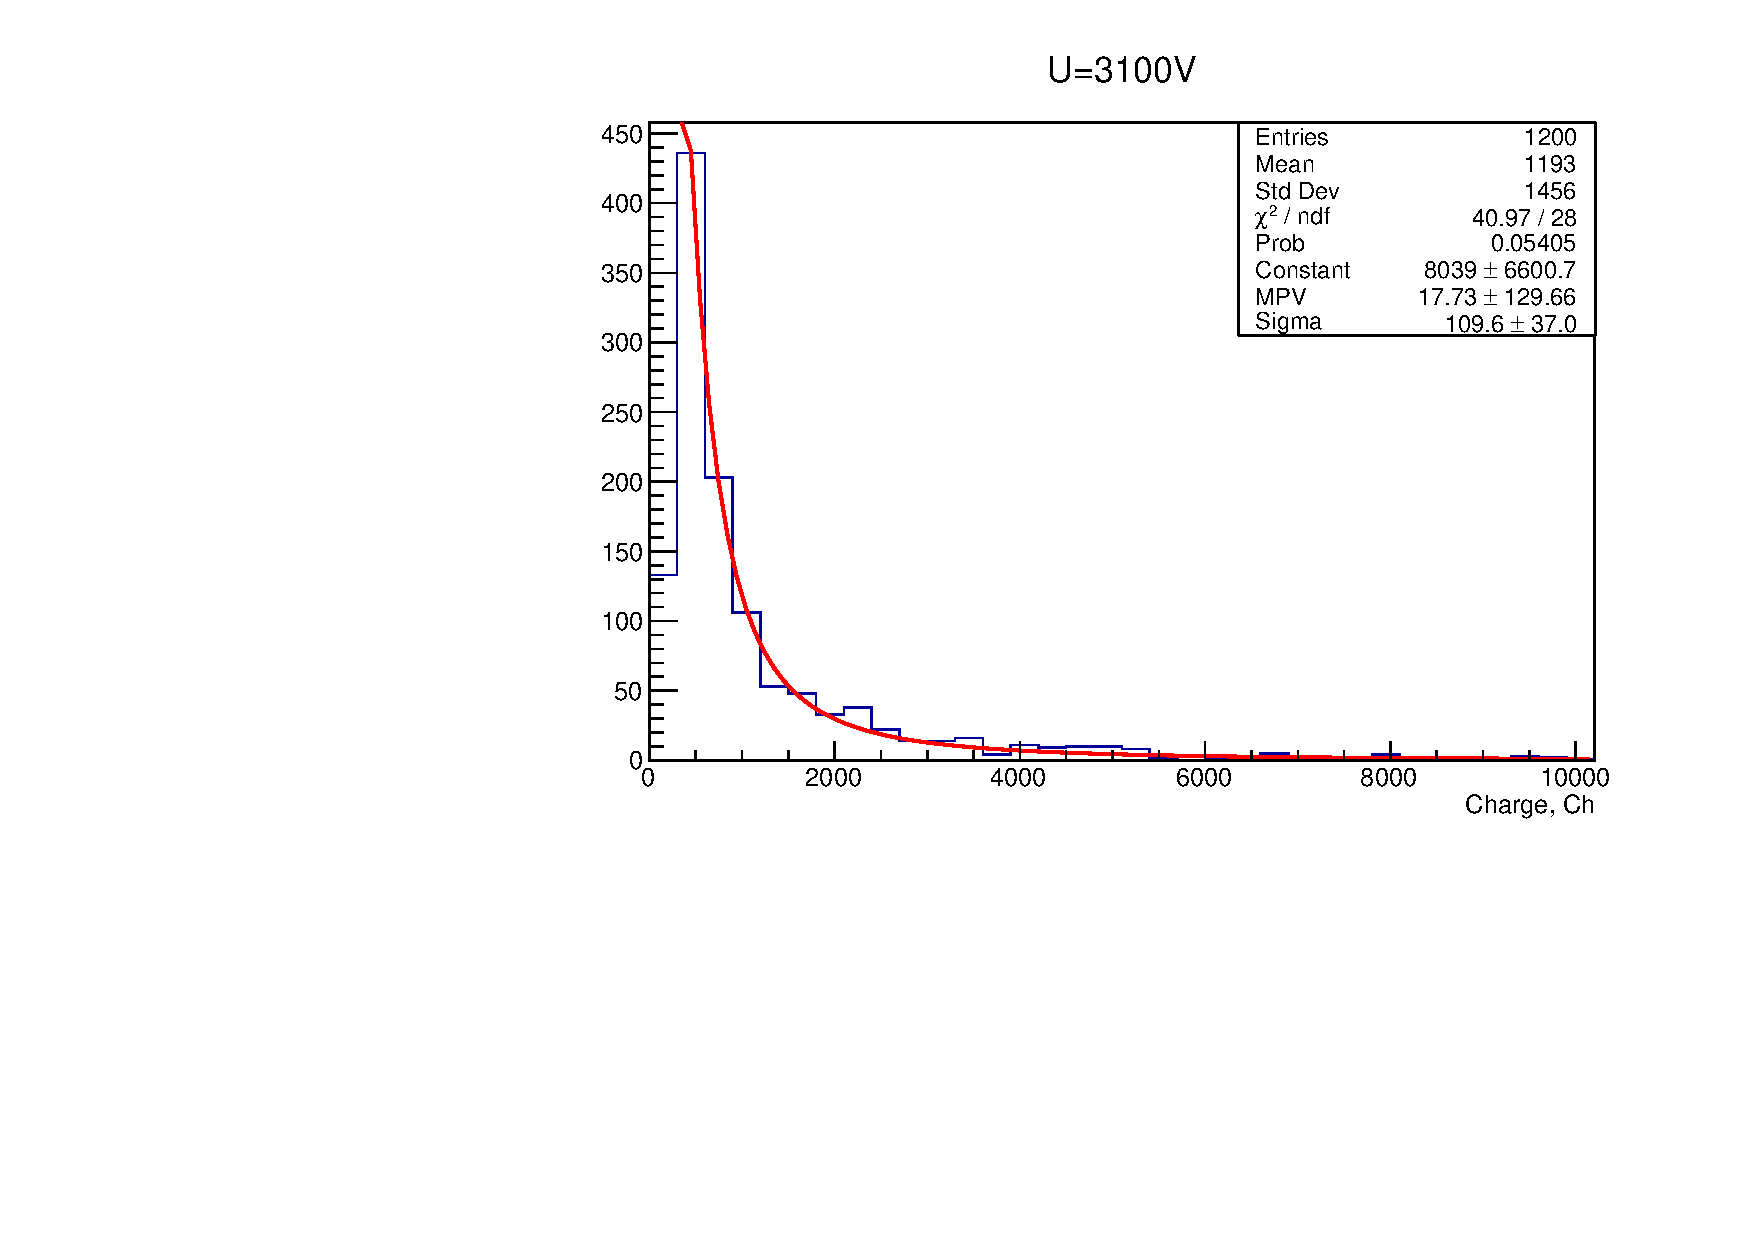
\includegraphics[width=1\linewidth]{img/3100.pdf}
	\caption{Напряжение на ускоряющей структуре 3100 В}
\end{subfigure}%
\hspace{20pt}
\begin{subfigure}{.45\textwidth}
	\centering
	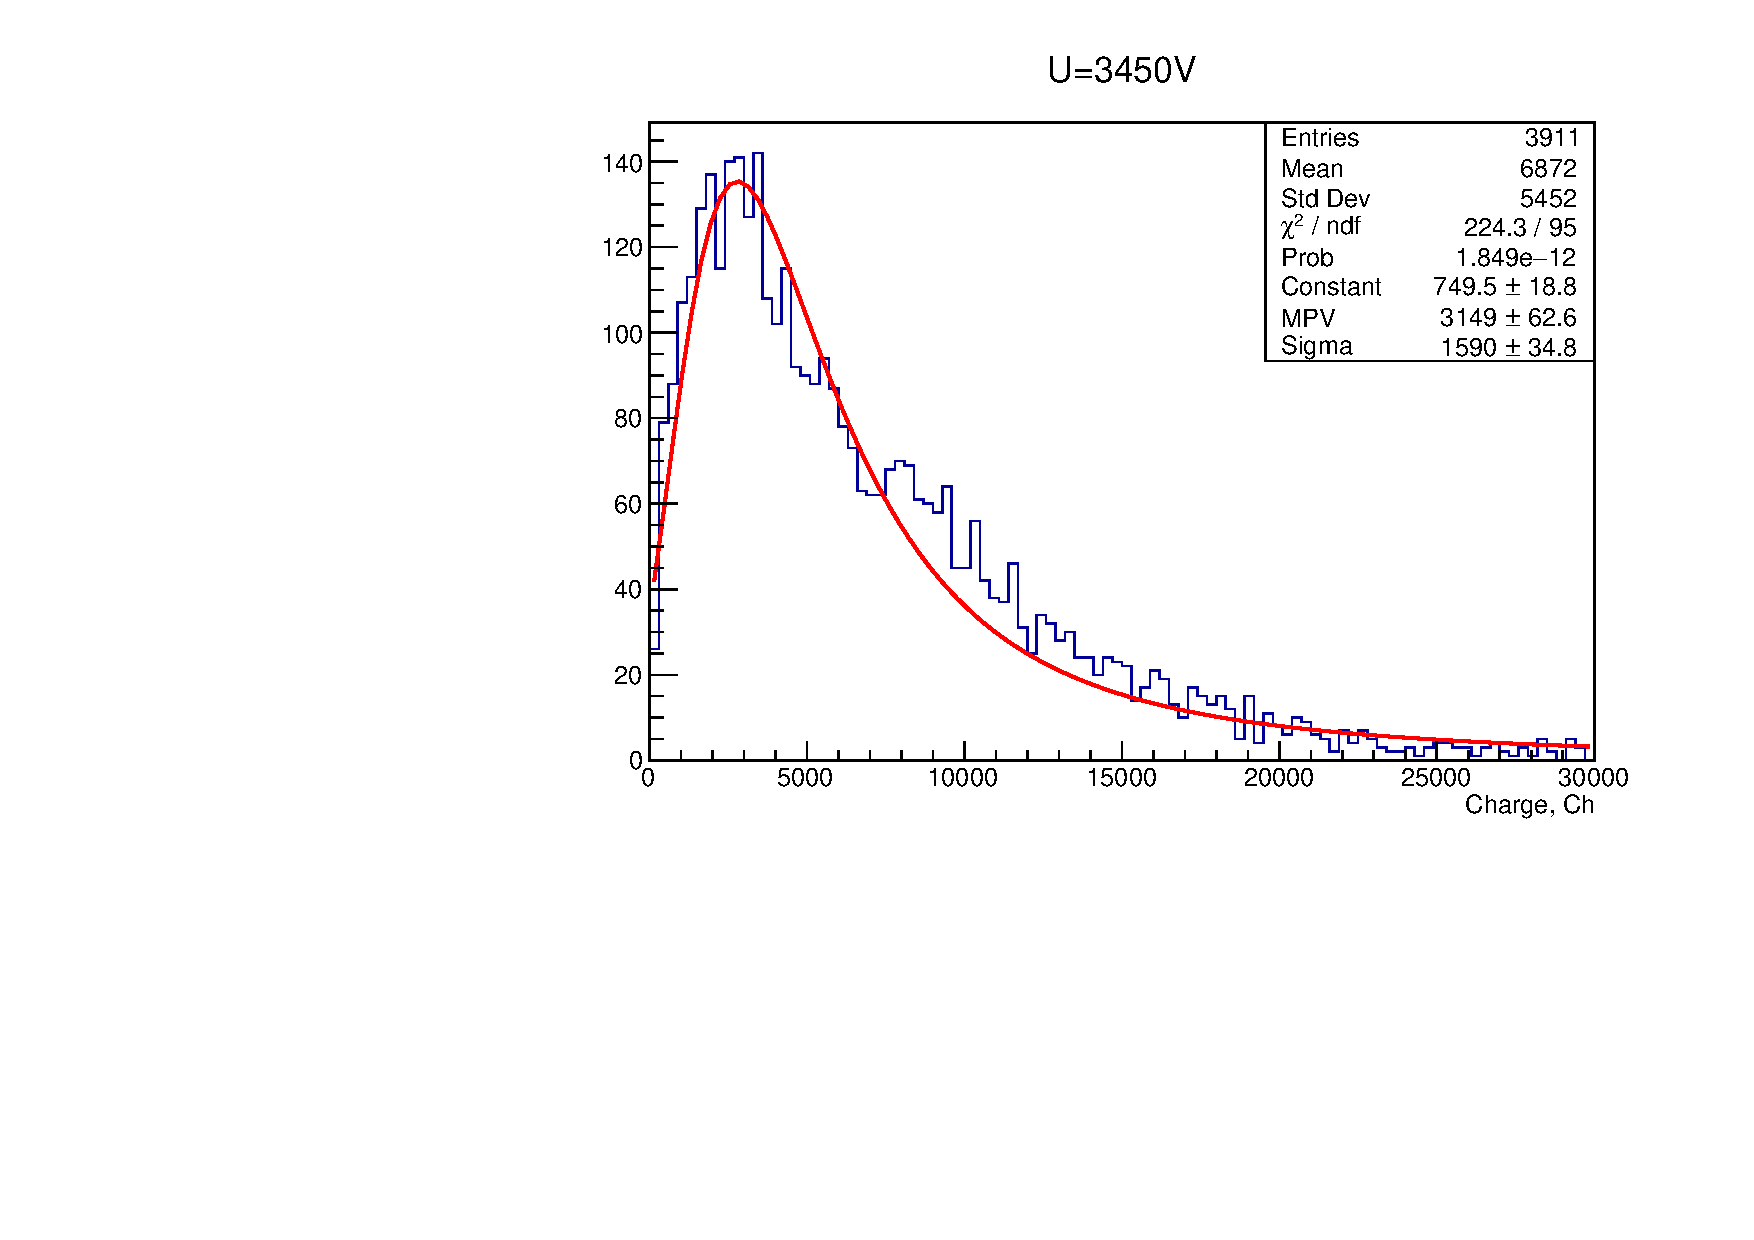
\includegraphics[width=1\linewidth]{img/3450.pdf}
	\caption{Напряжение на ускоряющей структуре 3450 В}
\end{subfigure}
\caption{Распределения по заряду кластера для разных значений напряжений на ускоряющей структуры детектора. Для напряжения 3100 В эффективность разделения сигнал--шум мала, поэтому положение пика распределения точно определить не получилось.}
\label{fig:charge_landau}
\end{figure}

\subsection{Результаты}
На Рис. \ref{fig:ampl_graph} представлены результаты измерений коэффициента усиления детектора. Для точек, где достоверно определен пик распределения Ландау наблюдается экспоненциальный тренд. Это указывает на правильную работу систем детектора.
\begin{figure}[h]
	\centering
	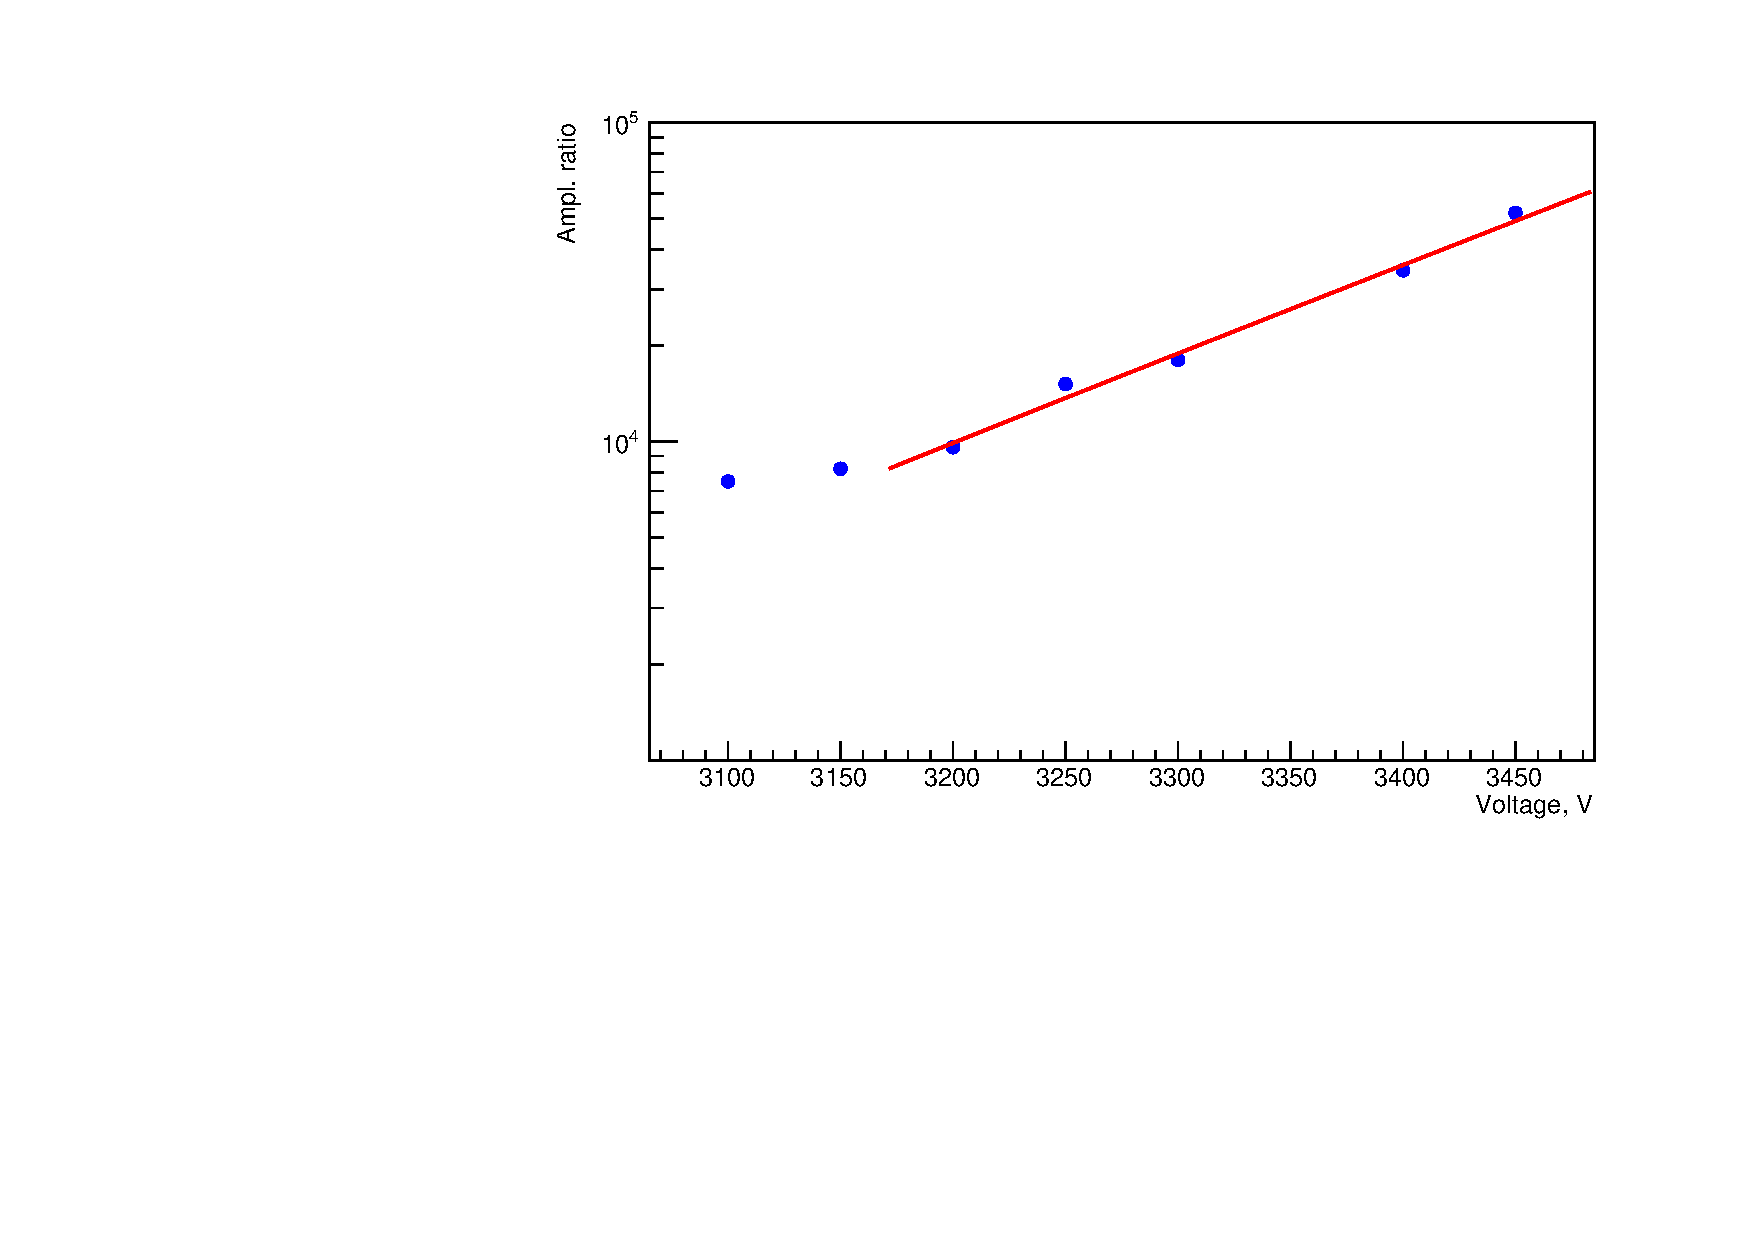
\includegraphics[width = 10cm]{img/Ampl_gr_log.pdf}
	\caption{Зависимость коэффициента усиления детектора от напряжения на ускоряющей структуре. Красная линия соответствует подгонке экспонентой.}
	\label{fig:ampl_graph}
\end{figure}
Максимальный коэффициент усиления, достигнутый при напряжении GEM--электродах 4500 В, составляет примерно 58000. Так же, при значении коэффициента усиления меньше 10000 достоверность разделения сигнала и шума резко уменьшается, что видно по количеству событий, отмеченных программой как сигнальные: при напряжении 3100 В было обработано 1200 сигнальных событий против 3900 при напряжении 3450 В. В точках с напряжением 3100 и 3150 В пик распределения Ландау был под границей шумов, поэтому его положение определялось лишь по правому склону распределения. Этим вызвана ошибка определения среднего заряда кластера, что привело к выполаживанию графика коэффициента усиления.

\section{Определение эффективности регистрации}
Еще одним параметром, который является ключевым для детектора, работающего в установке <<Лазерный поляриметр>>, является эффективность регистрации -- отношение числа зарегистрированных событий к их полному числу. Рассмотрим классическую схему для определения эффективности регистрации детекторов, которая подробно описана например в \cite{grupen}. Пусть имеется три детектора: D1, D2 и D3 с эффективностями $\varepsilon_1, \varepsilon_2$ и $\varepsilon_3$ соответственно. Требуется найти эффективность регистрации одного из них (для определенности выберем D1). Всего частиц, регистрируемых детекторами, $N_0$. Детекторы D2 и D3 необходимо включить в схему совпадений,т.е. сигнал о зарегистрированной частице должен генерироваться только тогда, когда они сработали одновременно. Это необходимо для эффективной фильтрации шумовых срабатываний. Схема из двух детекторов сможет зарегистрировать лишь $N_{23}$ событий. В предположении того, что акты регистрации частицы в двух детекторах абсолютно независимы, можно выразить $N_{23}$ как: 
\begin{equation}
N_{23} = \varepsilon_2\varepsilon_3 N_0.
\end{equation}
Если теперь добавить к этой схеме третий детектор и подсчитывать события, которые дали сигнал одновременно в трех детекторах, то их число будет: 
\begin{equation}
N_{123} = \varepsilon_1\varepsilon_2 \varepsilon_3 N_0.
\end{equation}
Отсюда можно определить эффективность регистрации третьего детектора: 
\begin{equation}
\varepsilon_1 = \frac{N_{123}}{N_{23}}
\end{equation}
Таким образом, для определения $\varepsilon_1$ необходимо знать количества событий, регистрируемых двумя схемами совпадений, одна из которых включает два детектора, а другая -- все три. Данный метод является простым и надежным, но не учитывает геометрических параметров детекторов, что так же может сильно повлиять на определяемое значение $\varepsilon$.
\subsection{Постановка эксперимента}
Измерение эффективности регистрации детектора <<Лазерного поляриметра>> было проведено на выведенном пучке электронов ускорителя ВЭПП-4М. Сначала был получен пучок тормозных гамма--квантов, которые затем конвертировались на свинцовой мишени в электрон--позитронные пары. Затем происходил отбор электронов по энергии с помощью спектрометрического магнита, за которым располагались детектирующая система.
 \begin{figure}[h]
 	\centering
 	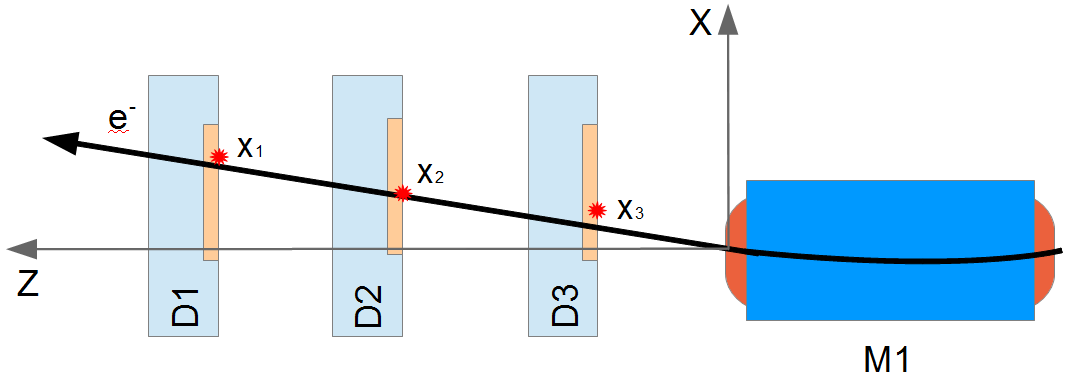
\includegraphics[width= 12cm]{img/reg_eff_exp_scheme.png}
 	\caption{Принципиальная схема установки для определения эффективности регистрации и пространственного разрешения на выведенном пучке ускорителя ВЭПП-4М. М1 -- спектрометрический магнит, D2,D3 -- вспомогательные детекторы, D1 -- исследуемый детектор.}
 	\label{fig:test_beam_scheme}
 \end{figure}
Для реализации схем совпадений помимо исследуемого детектора были использованы ещё два, которые работают в составе установки <<ДЕЙТОН>>. Это двухкоординатные GEM--детекторы с размером чувствительной области $160 \times 40$\,мм, применяемые на установке <<ДЕЙТОН>>. Все элементы схемы были позиционированы с помощью лазерных уровней и подключены к системе сбора данных выведенного пучка для того, чтобы получать сигналы триггера, который расположен сразу после мишени--конвертера. В ходе эксперимента тремя детекторами регистрировались координаты электронов выведенного пучка. Измерения проводились, начиная с напряжения на ускоряющей структуре 3200 В в шести точках с шагом 50 В. При последующей работе с данными события из разных детекторов связывались с помощью их порядкового номера в файлах. Стоит отметить, что данные, полученные при работе на выведенном пучке, были так же использованы для определения пространственного разрешения детектора. 

\subsection{Обработка и анализ результатов эксперимента}
Для удобства последующей работы на основе сырых данных были созданы деревья (ROOT TTree), которые содержали три ветви: две координаты и номер события. Для определения координат зарегистрированных частиц был программно реализован метод нахождения центра тяжести кластера. Его суть заключается в следующем: сначала определяются каналы, сигнал в которых превышает шумовой, затем по горизонтальной и вертикальной координате производится независимое суммирование вида: 
\begin{equation}
 \langle x \rangle = \frac{\sum_{i}q_i x_i}{\sum_{i}q_i},
\end{equation}
где $q_i$ -- заряд канала с координатой $x_i$. Нормировка производилось на полный заряд кластера.
\par По причине того, что чувствительная область детектора для поляриметра не охватывала весь пучок, стандартный алгоритм вычисления эффективности регистрации был модифицирован: в него добавлен учет геометрических параметров детектора и их влияние на конечную величину эффективности. Ниже приведена последовательность операций с данными для данного алгоритма.
\begin{itemize}
	\item Сначала отбирались события, попавшие в центральную область детектора <<Лазерного поляриметра>>
	\item Затем для этой выборки находились средние значения координат и дисперсии в дополнительных детекторах D2 и D3. 
	\item В детекторах D2 и D3 выделялись области с центром в точках, соответствующих средним значениям по выборке и размером в одно стандартное отклонение. 
	\item После этого \textit {по всему набору} подсчитывались события, которые попадают в выделенные области (в том числе и незарегистрированные исследуемым детектором.)
	\item Отношение числа событий из центральной области детектора <<Лазерного поляриметра>> к числу событий из выделенных областей дополнительных детекторов  регистрации. 
\end{itemize}

\subsection{Результаты}

\begin{figure}[h]
	\centering
	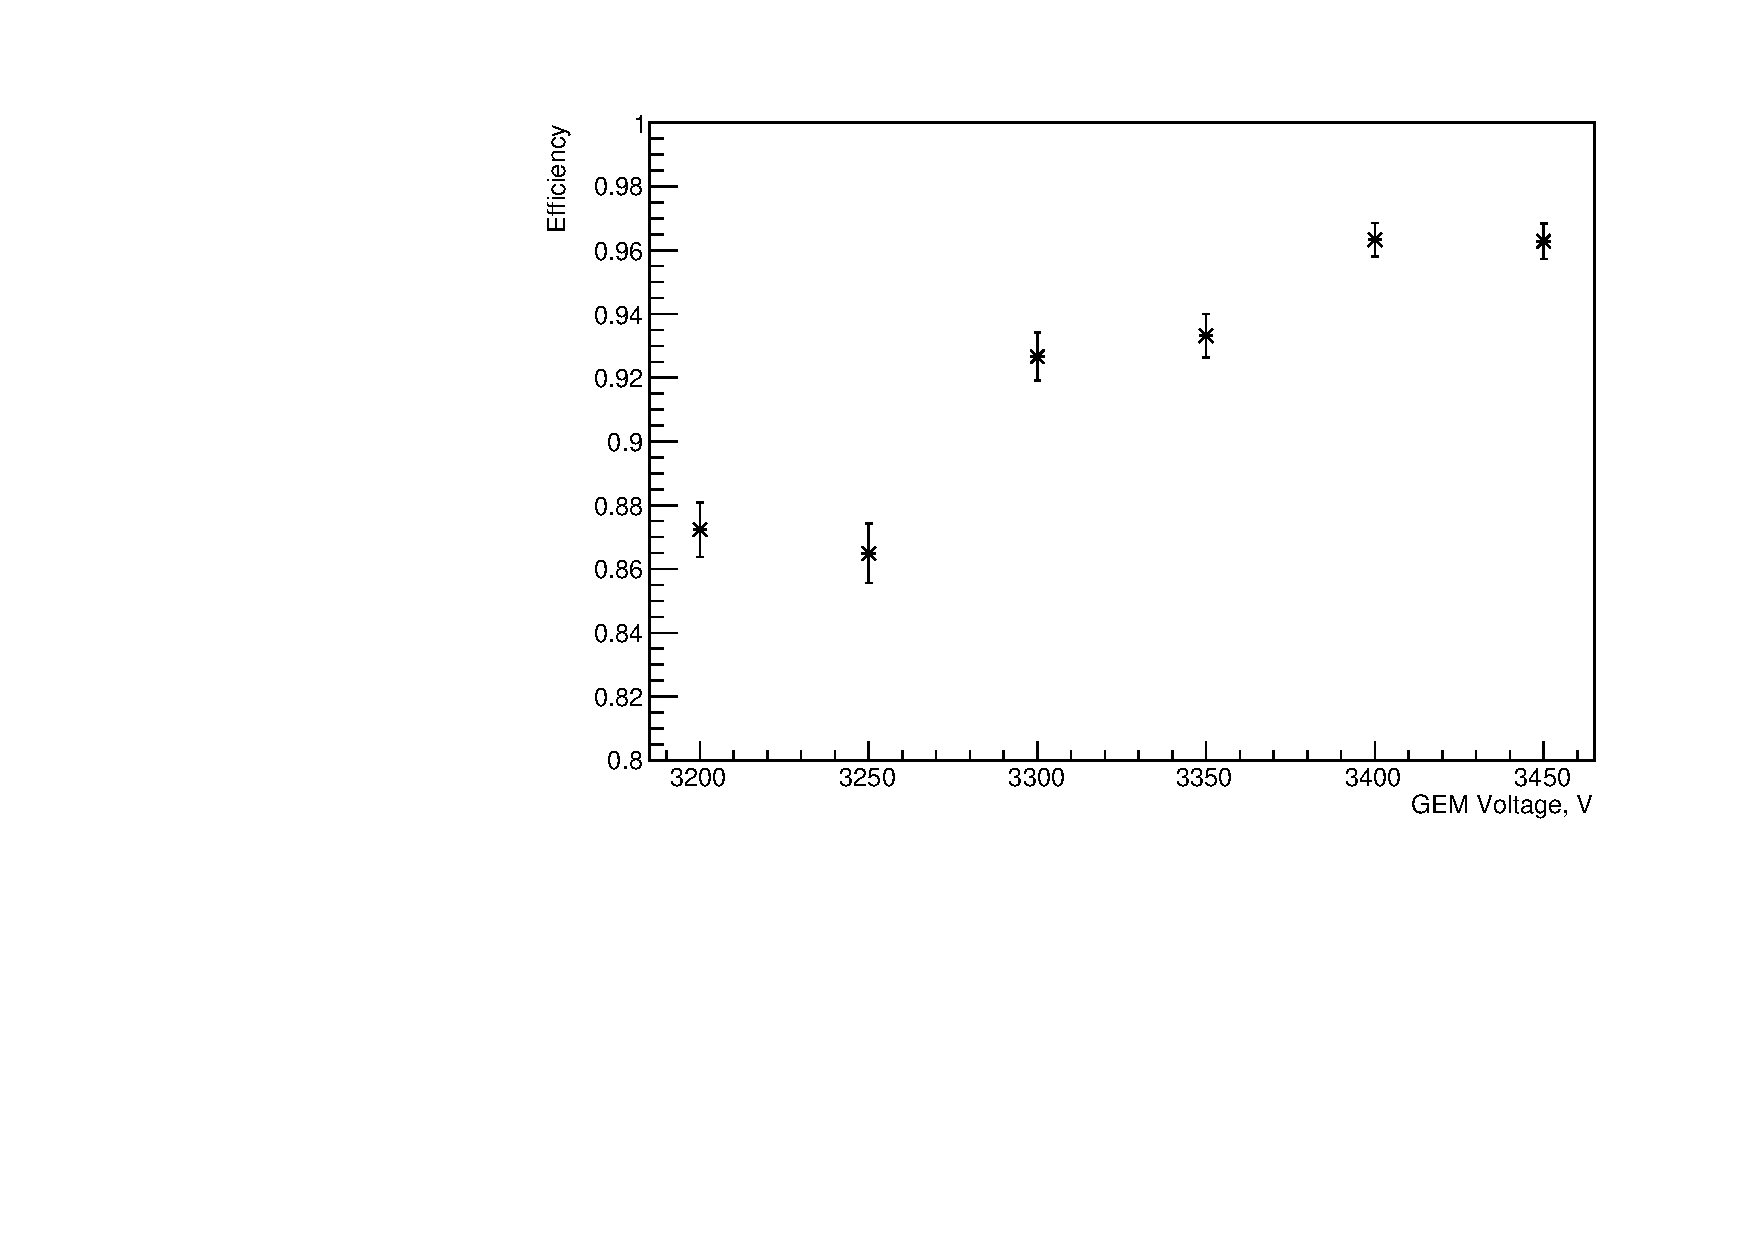
\includegraphics[width= 12cm]{img/eff_plot.pdf}
	\caption{Зависимость эффективности регистрации от напряжения на ускоряющей структуре.}
	\label{fig:eff_gr}
\end{figure}

\section{Определение пространственного разрешения}
\newpage
\bibliographystyle{include/utf8gost705u}
\bibliography{bibliography.bib}
\end{document}